\chapter{The Star Formation Rate at Galactic Scales: Theory}
\label{ch:sflaw_th}

\marginnote{
\textbf{Suggested background reading:}
\begin{itemize}
\item \href{http://adsabs.harvard.edu/abs/2014arXiv1402.0867K}{Krumholz, M.~R. 2014, Phys.~Rep., 539, 49}, section 4 \nocite{krumholz14c}
\end{itemize}
\textbf{Suggested literature:}
\begin{itemize}
\item \href{http://adsabs.harvard.edu/abs/2010ApJ...721..975O}{Ostriker, E.~C., McKee, C.~F., \& Leroy, A.~K. 2010, ApJ, 721, 975} \nocite{ostriker10a}
\item \href{http://adsabs.harvard.edu/abs/2013MNRAS.436.2747K}{Krumholz, M.~R. 2013, MNRAS, 436, 2747} \nocite{krumholz13c}
\end{itemize}
}

Chapter \ref{ch:sflaw_obs} was a brief review of the current state of the observations describing the correlation between star formation and gas in galaxies. This Chapter will focus on theoretical models that attempt to unify and make sense of these observations. To recap, there are a few broad observational results we would like any successful model to reproduce.
\begin{itemize}
\item Star formation appears to be a very slow or inefficient process, measured on both the galactic scale and the scale of individual molecular clouds (at least for local clouds). The depletion time is $\sim 100$ times larger than the free-fall time.
\item In unresolved observations, the rate of star formation appears to rise non-linearly with the total gas content.
\item In the central disks of galaxies, where most star formation takes place, star formation appears to correlate strongly with the molecular phase of the ISM, and poorly or not at all with the atomic phase.
\item The depletion time in molecular gas is nearly constant in nearby, ``normal" galaxies, though a weak dependence on total gas surface density cannot be ruled out given the observational uncertainties. In more actively star-forming galaxies with higher gas surface densities than any found within $\sim 20$ Mpc of the Milky Way, the depletion time does appear to be smaller.
\item  A correlation between star formation and atomic gas appears only in regions where the ISM is completely dominated by atomic gas, but with a very large scatter, and with a depletion time in the atomic gas is $\sim 2$ order of magnitude larger than that in molecular gas. In such regions, ``second parameters" such as the metallicity or the stellar mass density appear to affect the star formation rate in ways that they do not in inner disks.
\item If one uses tracers of higher density gas such as HCN, the depletion time is shorter than for the bulk of the molecular gas, but still remains much longer than any plausible estimate of the free-fall time in the emitting gas.
\end{itemize}
As we shall see, there is at present no theory that is capable of fully, self-consistently explaining all the observations. However, there are a number of approaches that appear to successfully explain at least some of the observations, and may serve as the nucleus for a fuller theory in the future.

\section{The Top-Down Approach}

Theoretical attempts to explain the correlation between gas and star formation in galaxies can be roughly divided into two categories: those that focus on regulation by galactic scale processes, and those that focus on regulation within individual molecular clouds. We will generically refer to the formers as ``top-down" models, and the latter as ``bottom-up" models.

\subsection{Hydrodynamics Plus Gravity}

The simplest approach to the problem of the star formation rate is to consider no physics beyond hydrodynamics and gravity, including no stellar feedback. Models with only these ingredients form a useful baseline against which more sophisticated models may be compared. A key question for such models is the extent to which large-scale gravitational instability is important. The importance of gravitational instability is determined by the \citet{toomre64a} $Q$ parameter, where
\begin{equation}
Q = \frac{\Omega \sigma}{\pi G \Sigma}
\end{equation}
where $\Omega$ is the angular velocity of the disk rotation, $\sigma$ is the gas velocity dispersion, and $\Sigma$ is the gas surface density. On your homework you will show that systems with $Q < 1$ are unstable to axisymmetric perturbations, while those with $Q>1$ are stable. Observed galactic disks appear to have $Q \approx 1$ over most of their disks, rising to $Q > 1$ at the edges of the disk.

\begin{marginfigure}
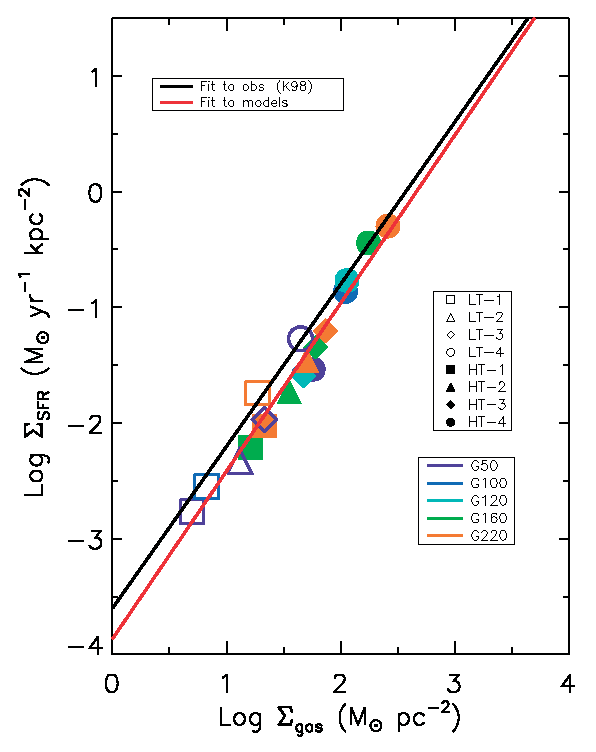
\includegraphics[width=\linewidth]{kslaw_sim_li05}
\caption[Kennicutt-Schmidt relation from simulations with only gravity and hydrodynamics]{
\label{fig:kslaw_sim_li05}
Relationship between gas surface density $\Sigma_{\mathrm{gas}}$ and star formation surface density $\Sigma_{\mathrm{SFR}}$, measured from a series of simulations using no physics except hydrodynamics and gravity \citet{li05a}.
}
\end{marginfigure}
If $Q \sim 1$, then gravitational instability occurring on galactic scales might be an important driver of star formation. If this is the case, then the rate of star formation is likely to be non-linearly sensitive to the value of $Q$, and thus to the gas surface density, potentially giving rise to the non-linear correlation between gas surface density and star formation rate seen in the unresolved observations. Some simulations are able to reproduce exactly this effect (Figure \ref{fig:kslaw_sim_li05}).

On the other hand, star formation can also occur even if $Q > 1$ and gravitational instability is unimportant on large scales, because in a multi-phase ISM there will still be places where the gas becomes locally cold and has $\sigma$ much less than the disk average. Such regions of dense, cold gas are expected to appear wherever the density is driven up by spiral arms or similar global structures. In this case we might expect that the star formation timescale should be proportional to the frequency with which spiral arms pass through the disk, and thus we should have
\begin{equation}
\Sigma_{\rm SFR} \propto \frac{\Sigma}{t_{\rm orb}},
\end{equation}
consistent with one of the observed parameterizations for galaxy-averaged star formation rates. In this approach, the key physics driving star formation is not the self-gravity of a galactic disk, but instead the ability of the gas to cool to low temperatures behind spiral shocks.

As a theory for the star formation rate, these models are mainly useful for target practice. (In fairness, they are often intended to study things other than the star formation rate, and thus make only minimal efforts to get this rate right.) We can identify a few obvious failings by comparing to our observational checklist. First of all, in these models, once gravitationally bound clouds form, there is nothing to stop them from collapsing in a timescale comparable to $t_{\rm ff}$. As a result, the star formation rate in molecular gas that these models predicts tends to be $\epsilon_{\rm ff} \sim 1$, rather than $\sim 0.01$, unless the models introduce an artificial means to lower the star formation rate -- in other words, this models produce rapid, efficient star formation rather than slow, inefficient star formation as required by the data. This is true even in the simulations with $Q>1$.

A second problem is that these models do not naturally predict any metallicity-dependence. Gravitational instability and large-scale spiral waves do not obviously care about the metallicity of the gas, but observations strongly suggest that metallicity does matter. It is possible that the interaction of spiral arms with cooling might give rise to a metallicity dependence in the star formation rate, but this has not be been explored.


\subsection{Feedback-Regulated Models}

\paragraph{Derivation}

The usual response to the failures of gravity plus hydro-only models has been to invoke ``feedback". The central idea for these models can be understood analytically quite simply. We begin by considering the gas momentum equation, ignoring viscosity but including magnetic fields:
\begin{equation}
\frac{\partial}{\partial t} (\rho\vecv) = - \nabla\cdot (\rho\vecv\vecv) - \nabla P + \frac{1}{4\pi} \nabla \cdot \left(\vecB\vecB - \frac{B^2}{2} \vecI\right) + \rho \vecg,
\end{equation}
where $\vecg$ is the gravitational force per unit mass, and the pressure $P$ includes all sources of pressure -- thermal pressure plus radiation pressure plus cosmic ray pressure. Let us align our coordinate system so that the galactic disk lies in the $xy$ plane. The $z$ component of this equation, corresponding to the vertical component, is simply
\begin{equation}
\frac{\partial}{\partial t} (\rho v_z) = - \nabla\cdot (\rho\vecv v_z) - \frac{dP}{dz} + \frac{1}{4\pi} \nabla \cdot \left(\vecB B_z\right) - \frac{1}{8\pi} \frac{d}{dz} B^2 + \rho g_z.
\end{equation}

Now let us consider some area $A$ at constant height $z$, and let us average the above equation over this area. The equation becomes
\begin{eqnarray}
\frac{\partial}{\partial t} \langle \rho v_z\rangle & = & -\frac{1}{A} \int_A \nabla\cdot (\rho\vecv v_z) \, dA - \frac{d\langle P\rangle}{dz} +
\frac{1}{4\pi A} \int_A \nabla \cdot \left(\vecB B_z\right)\, dA 
\nonumber \\
& & {} - \frac{1}{8\pi} \frac{d}{dz} \langle B^2 \rangle + \left\langle\rho g_z\right\rangle,
\end{eqnarray}
where for any quantity $Q$ we have defined
\begin{equation}
\langle Q\rangle \equiv \frac{1}{A}\int_A Q\, dA.
\end{equation}
We can simplify this a bit by separating the $x$ and $y$ components from the $z$ components of the divergences and making use of the divergence theorem:
\begin{eqnarray}
\frac{\partial}{\partial t} \langle \rho v_z\rangle & = & - \frac{d\langle P\rangle}{dz} - \frac{1}{8\pi} \frac{d}{dz} \langle B^2 \rangle + \left\langle\rho g_z\right\rangle  - \frac{d}{dz} \langle \rho v_z^2\rangle + \frac{1}{4\pi} \frac{d}{dz} \langle B_z^2\rangle \nonumber \\
& & {}- \frac{1}{A} \int_A \nabla_{xy}\cdot (\rho\vecv v_z) \, dA
\nonumber \\
& & {}  +
\frac{1}{4\pi A} \int_A \nabla_{xy} \cdot \left(\vecB B_z\right)\, dA \\
& = & - \frac{d\langle P\rangle}{dz} - \frac{1}{8\pi} \frac{d}{dz} \langle B^2 \rangle + \left\langle\rho g_z\right\rangle  - \frac{d}{dz} \langle \rho v_z^2\rangle + \frac{1}{4\pi} \frac{d}{dz} \langle B_z^2\rangle \nonumber \\
& & {}-\frac{1}{A} \int_{\partial A} v_z \rho \vecv \cdot \nhat \, d\ell + \frac{1}{4\pi A} \int_{\partial A} B_z \vecB \cdot \nhat \, d\ell.
\end{eqnarray}
where $\partial A$ is the boundary of the area $A$, and $\nhat$ is a unit vector normal to this boundary, which always lies in the $xy$ plane.

Now let us examine the last two terms, representing integrals around the edge of the area. The first of these integrals represents the advection of $z$ momentum $\rho v_z$ across the edge of the area. If we consider a portion of a galactic disk that has no net flow of material within the plane of the galaxy, then this must, on average, be zero. Similarly, the second integral is the rate at which $z$ momentum is transmitted across the boundary of the region by magnetic stresses. Again, if we are looking at a galactic disk in steady state with no net flows or advection in the plane, this must be zero as well. Thus the last two integrals are generally zero and can be dropped.

If we further assume that the galactic disk is approximately time steady, the time derivative is also obviously zero. We therefore arrive at an equation of hydrostatic balance for a galactic disk,
\begin{equation}
\frac{d}{dz} \left\langle P + \rho v_z^2 + \frac{B^2}{8\pi}\right \rangle  - \frac{d}{dz} \left\langle\frac{B_z^2}{4\pi}\right\rangle - \left\langle \rho g_z\right\rangle = 0
\end{equation}
The first term represents the upward force due to gradients in the total pressure, including the turbulent pressure $\rho v_z^2$ and the magnetic pressure $B^2/8\pi$. The third term represents the downward force due to gravity. The middle term represents forces due to magnetic tension, and is usually sub-dominant because it requires a special geometry to exert significant forces -- the field would need to be curved upward (think of a hammock) or downward (think of an arch) over most of the area of interest. Thus we are left with balancing the first and last terms.

The quantities in angle brackets can be thought of as forces, but they can equivalently be thought of as momentum fluxes. Each one represents the rate per unit area at which momentum is transported upward or downward through the disk, and in hydrostatic equilibrium these transport rates must match. The central \textit{ansatz} in the feedback-regulated model is to equate the rate of momentum transport represented by the first term with the rate of momentum injection by feedback. To be precise, one approximates that
\begin{equation}
\left \langle P + \rho v_z^2 + \frac{B^2}{8\pi}\right \rangle \sim \left\langle\frac{p}{M}\right\rangle \Sigma_{\rm SFR}
\end{equation}
where $\langle p/M\rangle$ is the momentum yield per unit mass of stars formed, due to whatever feedback processes we think are important. The quantity on the right hand side is the rate of momentum injection per unit area by star formation.

What follows from this assumption? To answer that, we have to examine the gravity term. For an infinite thin slab of material of surface density $\Sigma$, the gravitational force per unit mass above the slab is
\begin{equation}
g_z = 2\pi G \Sigma.
\end{equation}
Note that $\Sigma$ here should be the total mass per unit area within roughly 1 scale height of the mid-plane, including the contribution from both gas and stars. If we plug this in, then we get
\begin{equation}
\frac{d}{dz} \left(\left\langle \frac{p}{M}\right\rangle \Sigma_{\rm SFR}\right) \sim 2\pi G \Sigma
\quad \Longrightarrow \quad
\Sigma_{\rm SFR} \sim 2\pi G \left\langle \frac{p}{M}\right\rangle^{-1} \Sigma \Sigma_{\rm gas} ,
\end{equation}
where we have taken the vertical derivative $d/dz$ to be of order $1/h$, where $h$ is the gas scale height, and we have taken $\rho h \sim \Sigma_{\rm gas}$.

Thus in a feedback-regulated model, we expect a star formation rate that scales as the product of the gas surface density and the total surface density. In regions where gas dominates the gravity, so that $\Sigma \sim \Sigma_{\rm gas}$, we will have a star formation law
\begin{equation}
\Sigma_{\rm SFR} \propto \Sigma_{\rm gas}^2,
\end{equation}
while in regions where stars dominate we will instead have
\begin{equation}
\Sigma_{\rm SFR} \propto \Sigma_{\rm gas} \Sigma_*.
\end{equation}

To the extent that we think we know the momentum yield from star formation, $\langle p/M\rangle$, we can make the calculation quantitative and predict the actual rate of star formation, not just the proportionality. For example, estimates for the total momentum yield for supernovae give $\langle p/M\rangle \sim 3000$ km s$^{-1}$ by the end of the energy-conserving phase. Using this number, we obtain
\begin{equation}
\Sigma_{\rm SFR} \sim 0.09 M_\odot\mbox{ pc}^{-2}\mbox{ Myr}^{-1} \left(\frac{\Sigma}{100\,M_\odot\,\mathrm{pc}^{-2}}\right)^2,
\end{equation}
which is in the right ballpark for the observed star formation rate at that gas surface density.

A number of simulations of models of this type have been conducted, and they seem to show that one can indeed produce star formation rates that are in rough agreement with observation, for plausible choices of $\langle p/M\rangle$ and/or plausible implementations of stellar feedback. Figure \ref{fig:sffeedback_hopkins11} shows an example.

\begin{figure}
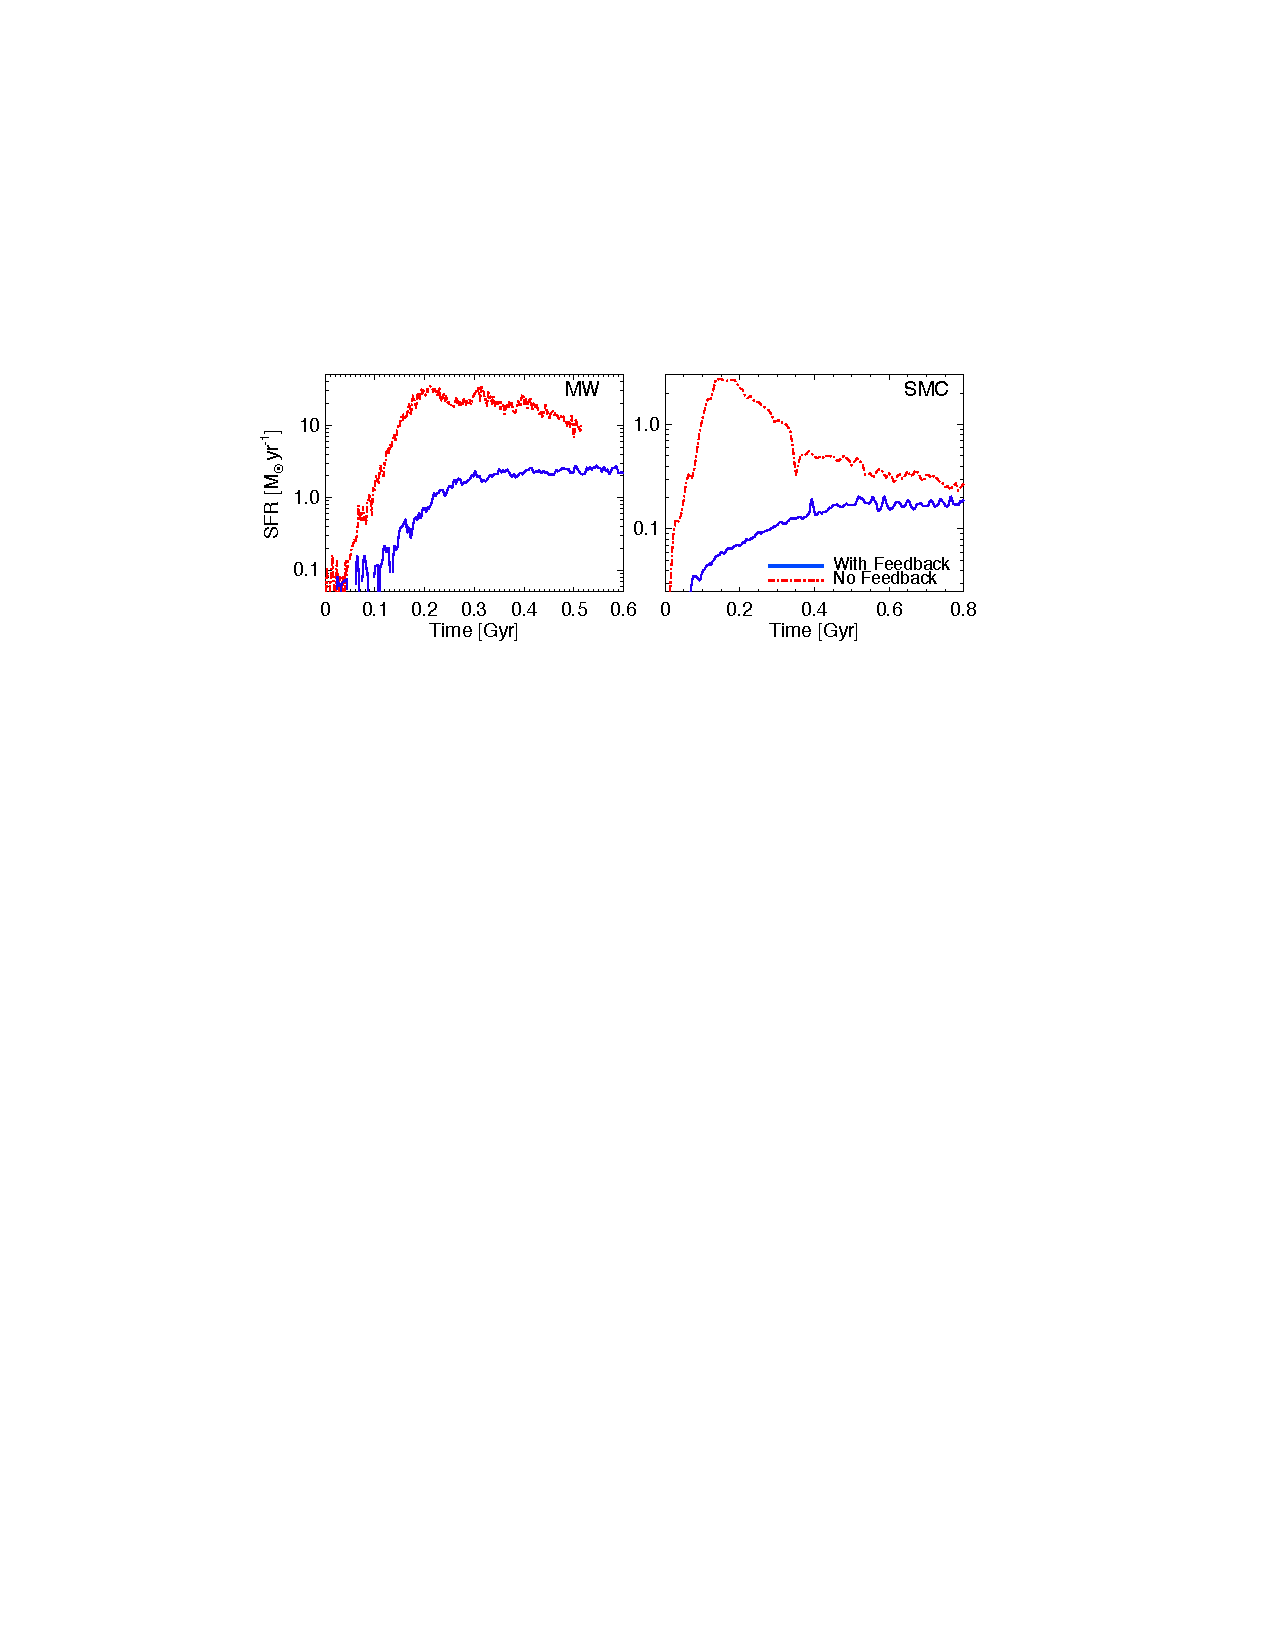
\includegraphics[width=\linewidth]{sffeedback_hopkins11}
\caption[Star formation rates in galaxy simulations with and without stellar feedback]{
\label{fig:sffeedback_hopkins11}
Star formation rates versus time measured in simulations of isolated galaxies performed with (blue) and without (red) a subgrid model for stellar feedback \citet{hopkins11a}. One simulation shown is for a galaxy with properties chosen to be similar to the Milky Way (left), and one is for a galaxy chosen to resemble the Small Magellanic Cloud (right).
}
\end{figure}

\paragraph{Successes and Failures of Feedback-Regulated Models}

Models of this sort have a number of appealing features. They are physically-motivated and allow quantitative calculation of the star formation rate, both in simulations and analytically. Another virtue of these models is that they allow one to calculate the star formation rate independent of any knowledge of how star formation operates within individual molecular clouds. Only the mean momentum balance of the ISM matters. This is particularly nice from the standpoint of simulations, because it means that one's choice of star formation recipe doesn't matter much to the results. A final virtue is that the linear scaling between $\Sigma_{\rm SFR}$ and $\Sigma_{\rm gas}$ expected in the regime where stars dominate the matter, and the scaling with stellar surface density, agree pretty well with what we see in outer galaxies.

However, there are also significant problems and omissions with this sort of model. First of all, the quantitative prediction is only as good as one's estimate of $\langle p/M\rangle$. As we have seen, there are significant uncertainties in this quantity.

Second, in models of this sort we expect to have $\Sigma_{\rm SFR} \propto \Sigma_{\rm gas}^2$ in the gas-dominated regime found in starburst galaxies. This is noticeably steeper than the observed scaling between $\Sigma_{\rm SFR}$ and $\Sigma_{\rm gas}$, which, as we have seen, has an index $\sim 1.5$. One can plausibly get this close to 2 by monkeying with the choice of $X_{\rm CO}$, but to push the index up to 2 requires pretty extreme choices.

Third, while this model goes a reasonable job of explaining how things might work in outer disks and why stars matter there, its predictions about the impact of metallicity appear to be in strong tension with the observations. Nothing in the argument we just made has anything to do with metallicity, and it is not at all clear how one could possibly shoehorn metallicity into this model. Thus the natural prediction of the feedback-regulated model is that metallicity does not matter. In contrast, as we discussed, the available evidence suggests quite the opposite.

A related issue is that it is not clear how atomic versus molecular gas fit into this story. All that matters in the global model is the weight of the ISM, which is unaffected by the chemical state of the gas, One could plausibly say that molecular gas simply forms wherever there is gas collapsing to stars, but then it is not clear why the depletion time in the molecular gas should be so much longer than the free-fall time -- if molecular gas is formed \textit{en passant} as atomic gas collapses to stars, why isn't it depleted on a free-fall time scale?

A fourth and final issue is that the independence of the predicted star formation rate on the local star formation law, which we praised as a virtue above, is also a defect. Observations appear to require that star formation be about as slow and inefficient within individual molecular clouds and dense regions as it is within galaxies as a whole. There are two independent lines of evidence to this effect: the low star formation rates measured in solar neighborhood clouds, and the correlation between infrared and HCN luminosity. However, in a feedback-regulated model there is no reason why this should be the case. Indeed, one can check this explicitly using simulations by changing the small scale star formation law used in the simulations (Figure \ref{fig:hcn-co_hopkins13}). If one changes the parameter describing how gas turns to stars within individual clouds, the star formation rate in the galaxy as a whole is unchanged, but the star formation rate within individual clouds, and the correlation between HCN emission and IR luminosity, changes dramatically.
\begin{marginfigure}
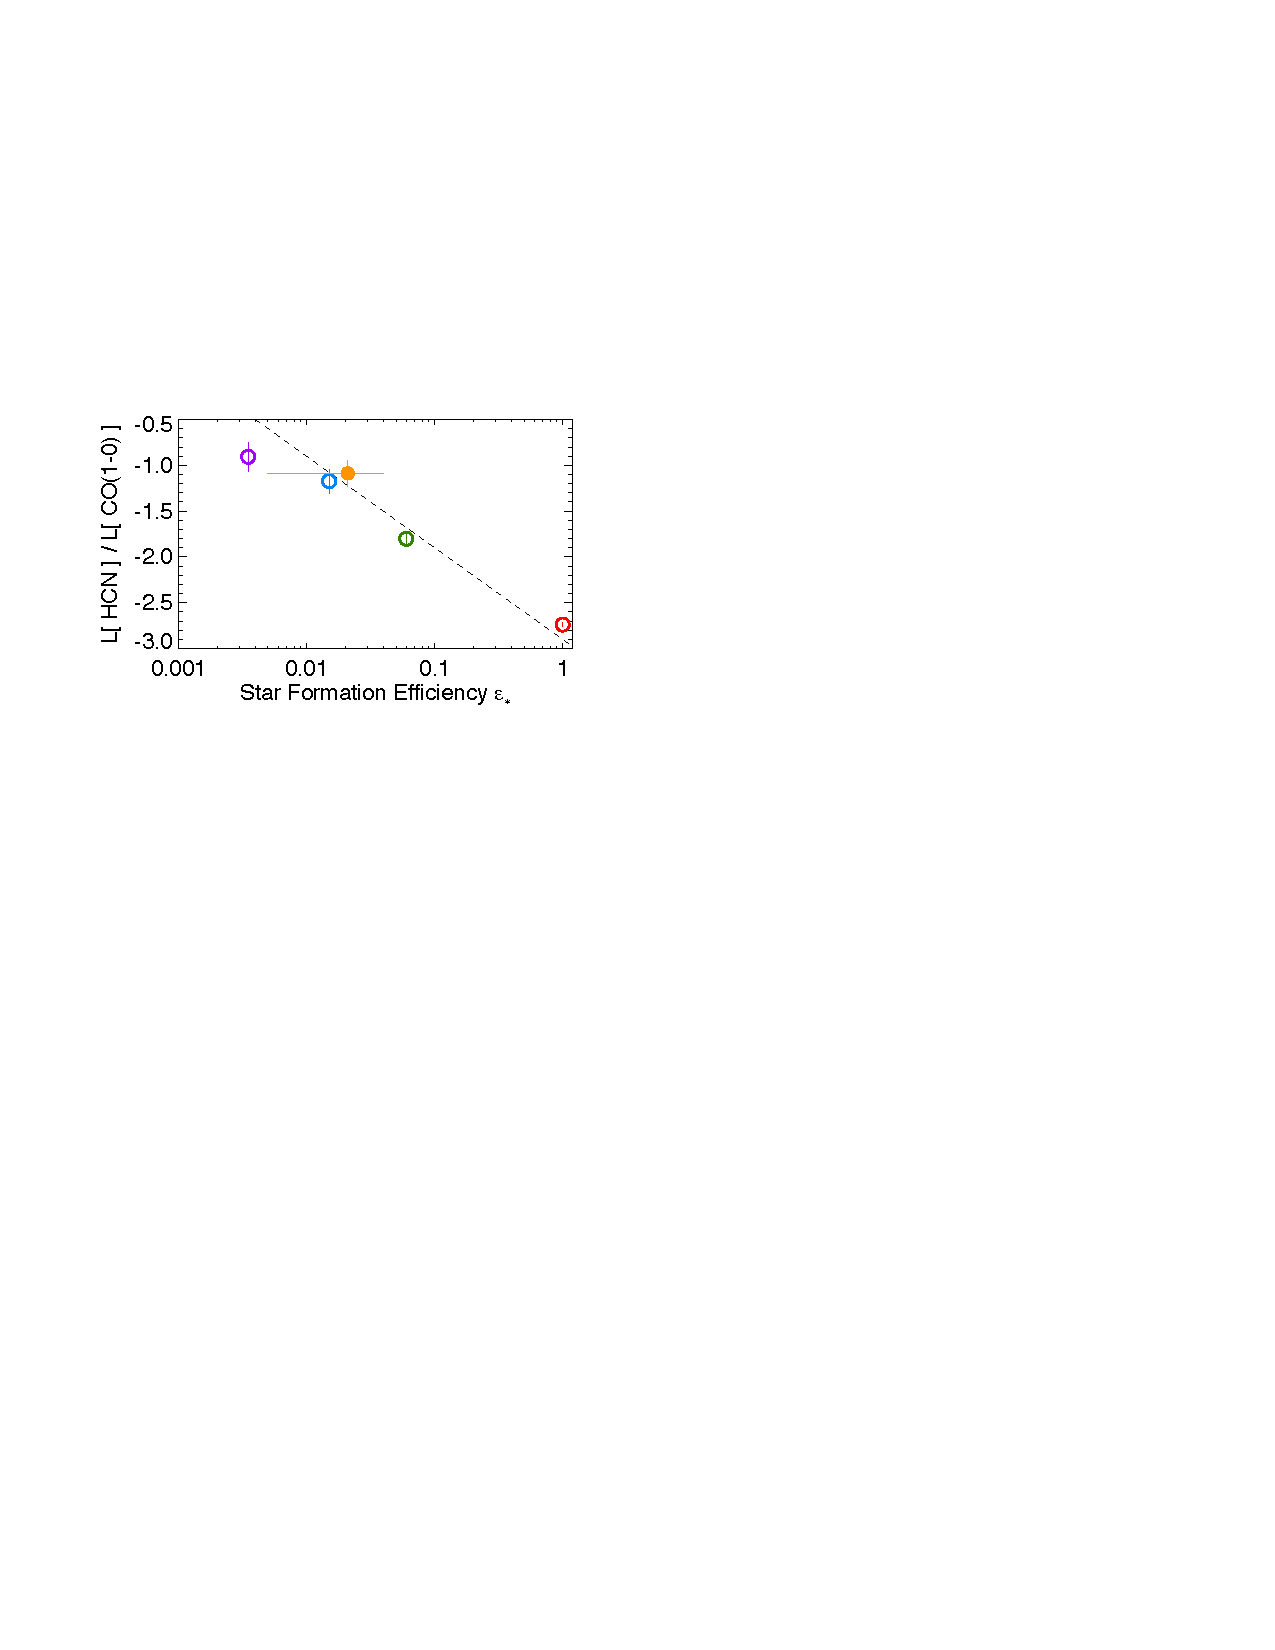
\includegraphics[width=\linewidth]{hcn-co_hopkins13}
\caption[Ratio of HCN to CO luminosity as a function of subgrid star formation recipe]{
\label{fig:hcn-co_hopkins13}
Ratio of HCN to CO luminosity computed from simulations of galaxies that are identical except for their subgrid model for the star formation rate in dense gas, parameterized by $\epsilon_*$ \citet{hopkins13c}.
}
\end{marginfigure}

One can sharpen the problem even more: in this story, the star formation rate is regulated primarily by feedback from massive stars. However, the star formation rate is observed to be low even in Solar neighborhood clouds where there are no stars larger than a few $M_\odot$, and where there probably will never be any because the stellar population is too small and low mass to be likely to produce any more massive stars. Why then is the star formation rate low in these clouds?

\section{The Bottom-Up Approach}

The alternate approach to the problem of the star formation rate has been to focus first on what happens inside individual clouds, and then to try to build up the galactic star formation law as simply the result of adding up lots of independent, small star-forming regions. The argument proceeds in two steps: first one attempts to determine which parts of the galaxy's ISM are ``eligible" to form stars, which under Milky Way-like conditions more or less reduces to the question how the ISM will be partitioned between a star-forming molecular phase and an inert atomic phase. The second step is to ask about the star formation rate within individual molecular clouds.

\subsection{Which Gas is Star-Forming?}

Observationally, stars form primarily or exclusively in molecular gas, and so it is natural to identify the star-forming part of the ISM with the molecular part. However, we would like to have a physical explanation for this correlation. The first explanation one might think of is that the formation of H$_2$ and CO lead to rapid cooling of the gas, allowing it to collapse. However, while CO is a very good coolant, it turns out that it is not much better than C$^+$, the main coolant in the cool atomic ISM. Moreover, in galaxies where there is a significant amount of H$_2$ that is not traced by CO, such as the Small Magellanic Cloud, star formation appears to correlate with the presence of H$_2$, not the presence of CO. This also suggests that CO cooling is not important.

Instead, the explanation that appears to have become accepted over the past few years is that H$_2$ is associated with star formation because of the importance of shielding. Let us recall the processes that set the thermal balance of the ISM. In a region without significant heating due to photoionization, the main heating processes are the grain photoelectric effect and cosmic ray heating. We can write the summed heating rate per H nucleus from both of these as
\begin{equation}
\Gamma = \left(4\times 10^{-26} \chi_{\rm FUV} Z'_d e^{-\tau_d} + 2\times 10^{-27} \zeta'\right) \mbox{ erg s}^{-1},
\end{equation}
where $\chi_{\rm FUV}$, $Z'_d$, and $\zeta'$ are the local FUV radiation field, dust metallicity, and cosmic ray ionization rate, all normalized to the Solar neighborhood value, and $\tau_d$ is the dust optical depth.

If we are in a region where the carbon has not yet formed CO, the main coolant will emission in the C$^+$ fine structure line at 92 K. This is fairly easy to compute. Assuming the gas is optically thin and well below the critical density (both reasonable assumptions), then the cooling rate is simply equal to the collisional excitation rate multiplied by the energy of the level, since every collisional excitation will lead to a radiative de-excitation that will remove energy. Thus we have a cooling rate per H nucleus
\begin{equation}
\Lambda_{\rm CII} = k_{\rm CII-H} \delta_C E_{\rm CII} n_{\rm H},
\end{equation}
where $k_{\rm CII-H} \approx 8\times 10^{-10} e^{-T_{\rm CII}/T}$ is the excitation rate coefficient, $T_{\rm CII} = 91$ K is the energy of the excited state measured in K, $\delta_C\approx 1.1\times 10^{-4} Z'_d$ is the carbon abundance relative to hydrogen, $E_{\rm CII} = k_B T_{\rm CII}$ is the energy of the level, and $n_{\rm H}$ is the hydrogen number density.

We can obtain the equilibrium temperature by setting the heating and cooling rates equal and solving. The result is
\begin{equation}
T = -\frac{T_{\rm CII}}{\ln \left( 0.36 \chi_{\rm FUV} e^{-\tau_d} + 0.018 \zeta'/Z'_d\right) - \ln n_{\rm H,2}},
\end{equation}
where $n_{\rm H,2} = n_{\rm H}/100$ cm$^{-3}$. Clearly there will be two possible behaviors of this solution, depending on whether the first or the second term in the logarithm dominates. If the first, FUV heating term, dominates, then we have
\begin{equation}
T \approx \frac{91\mbox{ K}}{1.0 + \tau_d - \ln \chi_{\rm FUV} + \ln n_{\rm H,2}}
\end{equation}
while if the second, cosmic ray term dominates, we have
\begin{equation}
T \approx \frac{91\mbox{ K}}{4.0 - \ln \zeta'/Z'_d + \ln n_{\rm H,2}}
\end{equation}
The transition between the two regimes occurs when $\tau_d \sim 3$.

In the cosmic ray-dominated regime, for $\zeta'/Z'_d = 1$ we get $T = 23$ K. Thus the gas can cool down to almost as low a temperature as we would get in a CO-dominated region (which will be closer to 10 K). On the other hand, if the cosmic ray heating rate is negligible compared to the FUV heating rate, and the optical depth is small, will have a temperature that is an order of magnitude higher than what we normally expect in molecular clouds. The corresponding Jeans mass,
\begin{equation}
M_J = \rho \lambda_J^3 = \rho \left(\frac{\pi c_s^2}{G \rho}\right)^{3/2} = 4.8\times 10^3\,M_\odot n_{\rm H}^{-1/2} T_2^{3/2}
\end{equation}
where $T_2 = T/100$ K, will differ between the two cases by a factor of $\sim (91/23)^{1.5} \approx 8$. Thus the presence of a high optical depth that suppresses FUV heating lowers the mass that can be supported against collapse by roughly an order of magnitude (or possibly more, if the local FUV radiation field is more intense than in the Solar neighborhood, as we would expect closer to the galactic center).

\begin{marginfigure}
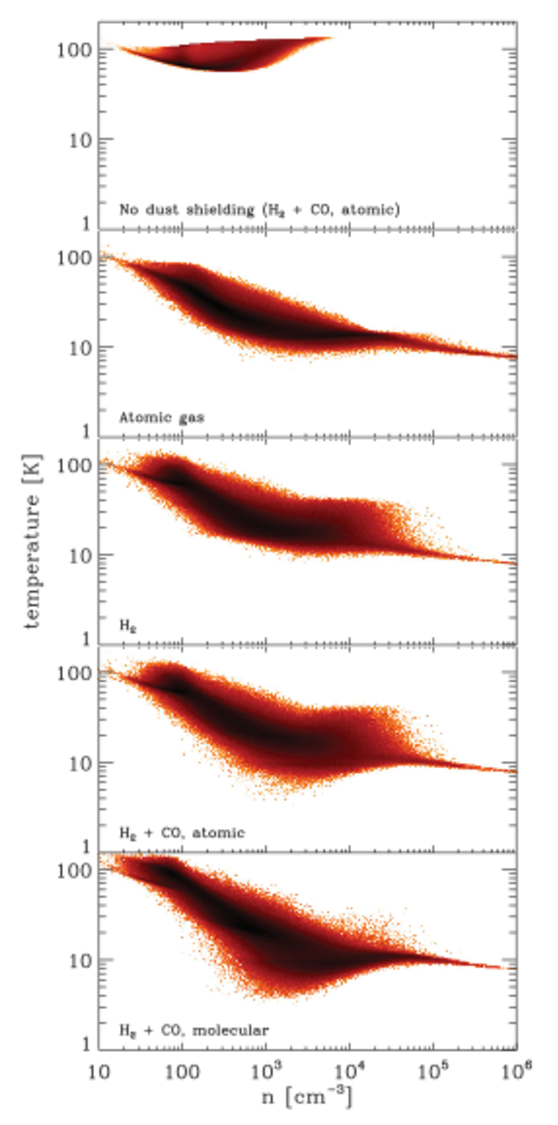
\includegraphics[width=\linewidth]{shielding_gc12}
\caption[Density-temperature distribution for different cooling models]{
\label{fig:shielding_gc12}
Density-temperature distributions measured in simulations with different treatments of ISM thermodynamics and chemistry \citet{glover12a}. All simulations use identical initial conditions, but vary in how the gas heating and cooling rates are calculated. The top panel ignores dust shielding, but includes full chemistry and heating and cooling. The bottom panel includes all chemistry and cooling. The middle three panels turn off, respectively, H$_2$ formation, CO formation, and CO cooling. The tail of material proceeding to high density in some simulations is indicative of star formation.
}
\end{marginfigure}

The central \textit{ansatz} in bottom-up models is that this dramatic change in Jeans mass has important implications for the regulation of star formation: in regions where the temperature is warm, the gas will be too thermally supported to collapse to form stars, while in regions where it gets cold star formation will proceed efficiently. There is some evidence for this from simulations (Figure \ref{fig:shielding_gc12}).

So what does all of this have to do with H$_2$? To answer that, recall that the transition to H$_2$ also depends critically upon shielding. We calculated earlier in the class that the shielding column of atomic hydrogen that has to be present before a transition to H$_2$ occurs is
\begin{equation}
N_{\rm H} = \frac{c f_{\rm diss} E_0^*}{n \mathcal{R}} \approx 7.5\times 10^{20} \chi_{\rm FUV} n_{\rm H,2}^{-1} (Z'_d)^{-1}\mbox{ cm}^{-2},
\end{equation}
or, in terms of mass surface density,
\begin{equation}
\Sigma = N_{\rm H} \mu m_{\rm H} = 8.4 \chi_{\rm FUV} n_{\rm H,2}^{-1} (Z'_d)^{-1}\,M_\odot\mbox{ pc}^{-2}.
\end{equation}

It is even more illuminating to write this in terms of the dust optical depth $\tau_d$. For FUV photons, the dust cross section per H nucleus is $\sigma_d \sim 10^{-21} Z'_d$ cm$^{-2}$, and so the dust optical depth one expects for the typical H~\textsc{i} shielding column is
\begin{equation}
\tau_d = N_{\rm H} \sigma_d = 7.5 \chi_{\rm FUV} n_{\rm H,2}^{-1} (Z'_d)^{-1}
\end{equation}
Thus the optical depth at which the gas becomes molecular is more or less the same optical depth at which the gas transitions from the FUV heating-dominated regime to the cosmic ray-dominated one. Moreover, Krumholz et al.~(2009) pointed out that the quantity $\chi_{\rm FUV} n_{\rm H,2}^{-1}$ appearing in these equations is not actually a free parameter -- in the main disks of galaxies where the atomic ISM forms a two-phase equilibrium, the cold phase will change its characteristic density in response to the local FUV radiation field, so that $\chi_{\rm FUV} n_{\rm H,2}^{-1}$ will always have about the same value (which turns out to be a few tenths).

Thus those models provide a natural, physical explanation for why star formation should be correlated with molecular gas, and why there is a turn-down in the relationship between $\Sigma_{\rm gas}$ and $\Sigma_{\rm SFR}$ at $\sim 10$ $M_\odot$ pc$^{-2}$. Gas that is cold enough to form stars is also generally shielded enough to be molecular, and vice versa. Gas that is not shielding enough to be molecular will also be too warm to form stars. The physical reason behind this is simple: the photons that dissociate H$_2$ are the same ones that are responsible for photoelectric heating, so shielding against one implies shielding against the other as well. Detailed models reproduce this qualitative conclusion (e.g., \citealt{krumholz11b}).

This model also naturally explains the observed metallicity-dependence of both the H~\textsc{i} / H$_2$ transition and the star formation. With a bit more work, it can also explain the linear dependence of $\Sigma_{\rm SFR}$ and $\Sigma_{\rm gas}$ in the H~\textsc{i}-dominated regime -- in essence, once one gets to the regime of very low star formation and weak FUV fields, the quantity $\chi_{\rm FUV} n_{\rm H,2}^{-1}$ can't stay content any more, because $n_{\rm H,2}$ can't fall below the minimum required to maintain hydrostatic balance. This puts a floor on the fraction of the ISM that is dense and shielded enough to form stars, which is linearly proportional to $\Sigma_{\rm gas}$. Figure \ref{fig:kshi_krumholz13} shows the result.

\begin{figure}
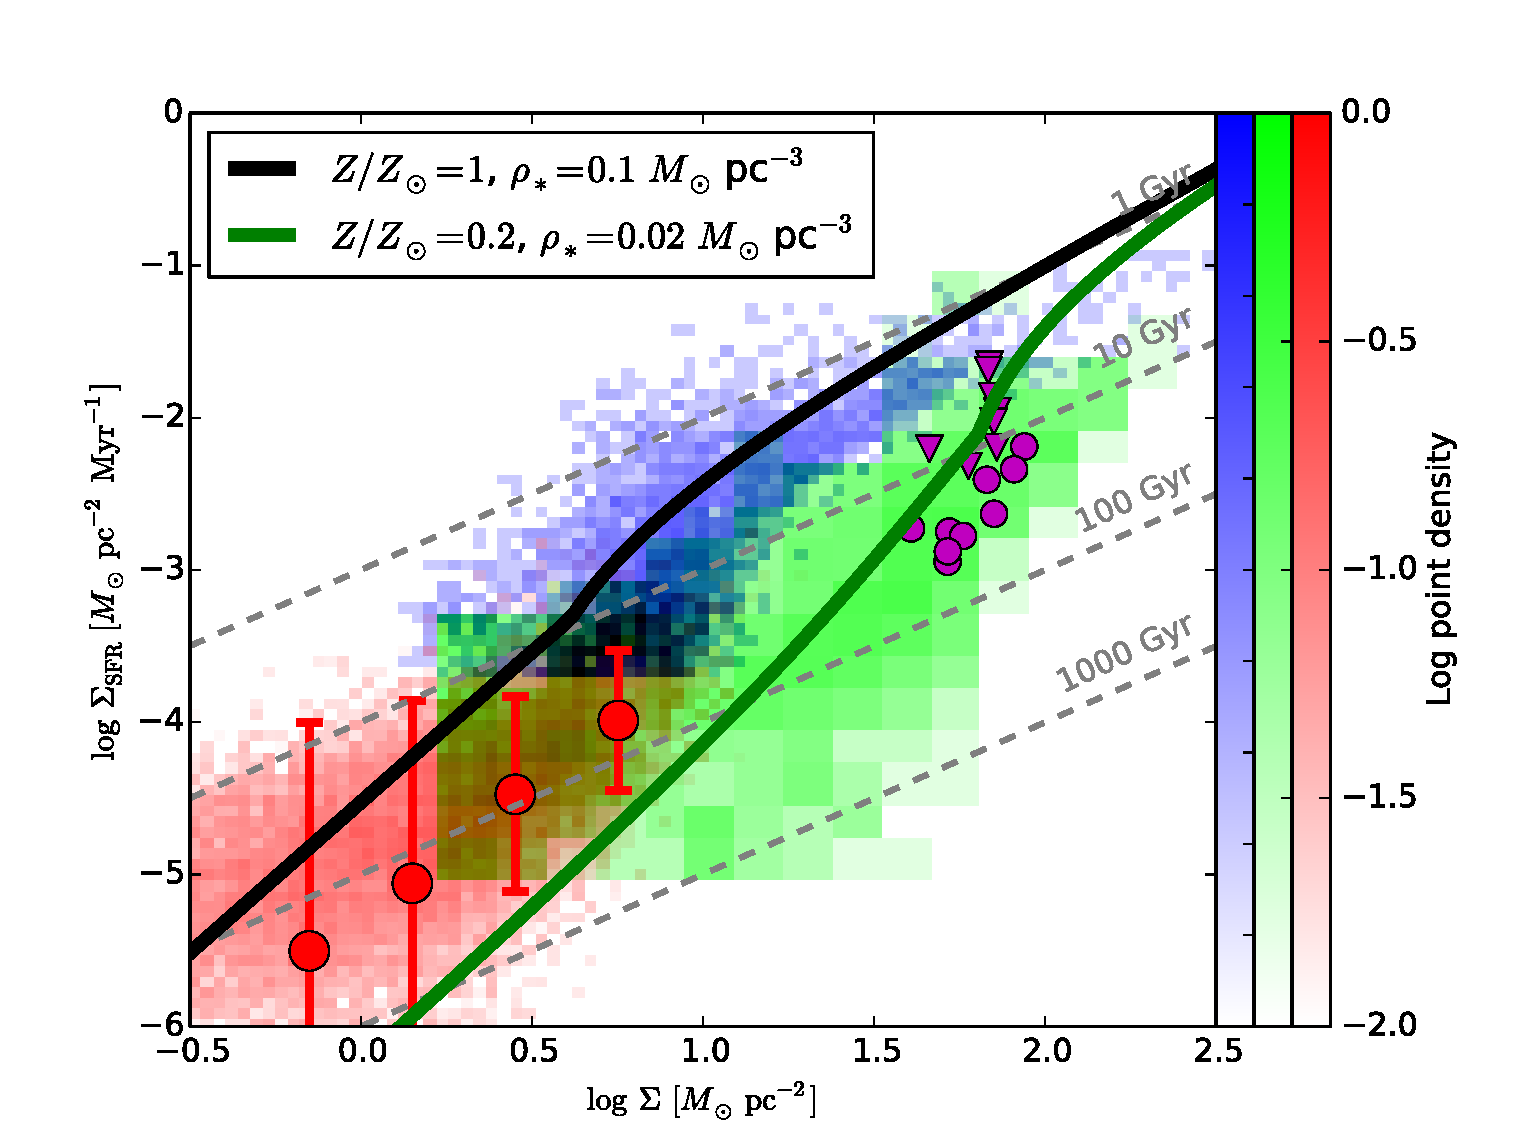
\includegraphics[width=\linewidth]{kshi_krumholz13}
\caption[Theoretical model for metallicity-dependence of the star formation rate]{
\label{fig:kshi_krumholz13}
Relationship between star formation rate surface density $\Sigma_{\mathrm{SFR}}$ and total gas surface density $\Sigma$. Pixels and points show observations, and are the same as in Figure \ref{fig:kstot_krumholz14}. Solid black and green lines are theoretical models from \citet{krumholz13c} for two different combinations of metallicity normalized to Solar, $Z/Z_\odot$, and mid-plane stellar density, $\rho_*$, as indicated in the legend.
}
\end{figure}

\subsection{The Star Formation Rate in Star-Forming Clouds}

Thus far the model we have outlined explains the metallicity-dependence and the overall shape of the relationship between total gas and star formation, but it does not say anything about the overall rate of star formation in molecular regions. Why is the star formation rate in molecular gas so low?

One potential explanation focuses on the role of turbulent support. This model was first developed quantitatively by \citet{krumholz05c}, and has subsequently been refined and improved by a large number of authors (e.g., \citealt{hennebelle11b, padoan11a, padoan14a, federrath12a}). The argument is fairly simple, and it relies on the statistical properties of the turbulence we've already discussed. Consider a turbulent medium with a linewidth-size relation
\begin{equation}
\sigma(l)=c_s\left(\frac{l}{\lambda_s}\right)^{1/2},
\end{equation}
where $c_s$ is the sound speed and $\lambda_s$ is the sonic length. We want to know what parts of this flow will go Jeans-unstable and begin to collapse. The maximum mass that can held up against turbulence is the Bonnor-Ebert mass, which you will calculate for homework:
\begin{equation}
M_{\rm BE} = 1.18 \frac{c_s^3}{G^3\rho} = \frac{1.18}{\pi^{3/2}}\rho \lambda_J^3,
\end{equation}
where $c_s$ is the isothermal sound speed and $\rho$ is the {\it local} gas density, i.e.\ the density at the surface of the Bonnor-Ebert sphere. The corresponding radius is
\begin{equation}
R_{\rm BE} = 0.37\lambda_J
\end{equation}
Let's evaluate the various terms in the virial theorem for this object. The gravitational energy is
\begin{equation}
\mathcal{W} = -a \frac{G M_{\rm BE}^2}{R_{\rm BE}} = -1.06 \frac{c_s^5}{G^{3/2} \rho^{1/2}},
\end{equation}
where $a$ is a geometric factor that depends on the density distribution, and for the numerical evaluation we used $a=0.73$, the numerical value for a maximum mass Bonnor-Ebert sphere. The corresponding thermal energy is
\begin{equation}
\mathcal{T}_{\rm th} = \frac{3}{2}M_{\rm BE} c_s^2 = 1.14 |\mathcal{W}|.
\end{equation}
Finally, to estimate the turbulent energy we'll use the linewidth-size relation, and assume that the velocity dispersion is given by $\sigma(2 R_{\rm BE})$, i.e. by the linewidth-size relation evaluated at a length scale equal to diameter of the sphere. This gives
\begin{equation}
\mathcal{T}_{\rm turb} = \frac{3}{2} M_{\rm BE} \sigma(2R_{\rm BE})^2 = 0.89 \left(\frac{\lambda_J}{\lambda_s}\right) |\mathcal{W}|.
\end{equation}
More sophisticated treatments, as given in some of the papers cited above, include magnetic support as well. For simplicity, though, we'll omit there here.

Now let's turn this around and hypothesize that the collapsing parts of the flow are those for which the density is unusually high, such that potential energy is comparable to or larger than the turbulent energy. Based on what we just calculated, for this condition to be true it must be the case that the local Jeans length $\lambda_J$ is comparable to or smaller than the sonic length $\lambda_s$.

As an ansatz, we therefore say that collapse will occur in any region where $\lambda_J \lesssim \lambda_s$. It is convenient to write this in terms of the Jeans length at the mean density
\begin{equation}
\lambda_{J0}=\sqrt{\frac{\pi c_s^2}{G\overline{\rho}}},
\end{equation}
where $\overline{\rho}$ is the mean density.
If we let $x = \rho/\overline{\rho}$, then $\lambda_J = \lambda_{J0}/\sqrt{x}$. The condition that $\lambda_J \lesssim \lambda_s$ therefore requires that the overdensity $x$ satisfy
\begin{equation}
x > x_{\rm crit} \equiv \left(\phi_x \frac{\lambda_{J0}}{\lambda_s}\right)^2,
\end{equation}
where we have replaced the $\lesssim$ simply with a firm inequality, and introduced $\phi_t$, a dimensionless number of order unity.

The nice thing is that we can now determine what fraction of the mass satisfies this condition simply from knowing the density PDF:
\begin{eqnarray}
f & = & \int_{x_{\rm crit}}^\infty \frac{dp}{d\ln x} dx \\
& = & \frac{1}{\sqrt{2\pi \sigma_{\rho}^2}}
\int_{x_{\rm crit}}^\infty \exp\left[-\frac{(\ln x - \overline{\ln x})^2}{2\sigma_{\rho}^2}\right] \, dx \\
& = & \frac{1}{2} \left[1+\mbox{erf}\left(\frac{-2\ln x_{\rm crit}+\sigma_{\rho}^2}{2^{3/2}\sigma_{\rho}}\right)\right],
\end{eqnarray}
where $\sigma_{\rho} \approx [\ln(1+3\mathcal{M}^2/4)]^{1/2}$ and $\mathcal{M}$ is the 1D Mach number.
If we then hypothesize that a fraction $\sim f$ of the cloud will collapse every cloud free-fall time, the total star formation rate per free-fall time in the simulations should follows
\begin{equation}
\epsilon_{\rm ff} = \frac{1}{2 \phi_t} \left[1+\mbox{erf}\left(\frac{-2\ln x_{\rm crit}+\sigma_{\rho}^2}{2^{3/2}\sigma_{\rho}}\right)\right],
\end{equation}
where $\phi_t$ is another fudge factor of order unity.

Another assumption here is that the collapse time is given by the global free-fall time, as opposed to a density-dependent local free-fall time. Again, this is an area where subsequent work by Hennebelle \& Chabrier and Federrath \& Klessen have improved on the original model. It turns out to be a better assumption that the collapse happens on a local free-fall timescale instead, in which case we instead have a star formation rate
\begin{equation}
\epsilon_{\rm ff} = \frac{1}{\phi_t} \int_{x_{\rm crit}}^\infty \frac{dp}{d\ln x} x^{1/2} \, dx
= \frac{1}{2\phi_t} \left[1+\mbox{erf}\left(\frac{-\ln x_{\rm crit}+\sigma_{\rho}^2}{2^{1/2}\sigma_{\rho}}\right)\right] \exp\left(\frac{3}{8}\sigma_\rho^2\right),
\end{equation}
where the extra factor of $x^{1/2}$ inside the integral comes from the fact that $t_{\rm ff} \propto \rho^{-1/2}$, so higher density regions get weighted more because they collapse faster.

We can write the critical ratio $\lambda_{J0}/\lambda_s$ in terms of quantities that we can determine by observations. If we have a region for which the virial ratio is
\begin{equation}
\avir = \frac{5\sigma^2 R}{GM},
\end{equation}
with $\sigma$ here representing the velocity dispersion over the entire region, then the linewidth-size relation is
\begin{equation}
\sigma(l) = \sigma_{\rm 2R} \left(\frac{l}{2R}\right)^{1/2}.
\end{equation}
We therefore have
\begin{equation}
\lambda_s = 2R \left(\frac{c_s}{\sigma_{2R}}\right)^2.
\end{equation}
Similar, we can re-write the mean-density Jeans length as
\begin{equation}
\lambda_{J0} = \sqrt{\frac{\pi c_s^2}{G\overline{\rho}}} = 2\pi c_s \sqrt{\frac{R^3}{3 GM}}.
\end{equation}
Putting this together, we get
\begin{equation}
x_{\rm crit} = \left(\phi_x \frac{\lambda_{J0}}{\lambda_s}\right)^2 = \frac{\pi^2 \phi_x^2}{15} \avir \mathcal{M}^2 \approx 0.82\avir \mathcal{M}^2.
\end{equation}
Since $\epsilon_{\rm ff}$ is a function only of $x_{\rm crit}$ and $\sigma_{\rho}$, and these are now both known in terms of $\avir$ and $\mathcal{M}$, we have now written the star formation rate in terms of $\avir$ and $\mathcal{M}$. Numerical evaluation is straightforward, and full 3D simulations show that the theory works reasonably well \citep{federrath12a}. 

For $\alpha_{\rm vir} \sim 2$, comparable to observed values, the numerical value of $\epsilon_{\rm ff}$ typically comes out a bit too high compared to observations, closer to $\sim 0.1$ than $\sim 0.01$, but localized sources of feedback like protostellar outflows are likely able to reduce that further. Such feedback would be required in any event, since without it the turbulence would decay and the star formation rate would rise.

\subsection{Strengths and Weaknesses of Bottom-Up Models}

Comparing the bottom-up models to our observational constraints, we see that they do better than the top-down ones on some metrics, not quite as well on others. As already mentioned, the bottom up models naturally reproduce the observed dependence of star formation on the phase of the ISM, and on the metallicity. This is a major difference from the top-down models, which struggle on these points.

A second strength of the bottom-up model, at least one in which turbulence is assumed to regulate the star formation rate within molecular clouds, is that it automatically reproduces the observation that $\epsilon_{\rm ff} \sim 0.01$ on \textit{all scales}, from individual clouds to small dense regions to entire galaxies; indeed, the central assumption of the model is that the galactic star formation law is simply a sum of local cloud ones. Thus the local-global connection is made naturally.

However, the model has two major weaknesses as well. First, the explanation why $\epsilon_{\rm ff} \sim 0.01$, as opposed to $\sim 0.1$, is still somewhat hazy, and relies on generalized appeals to local feedback processes that are not tremendously well understood. The central problem is that of dynamic range. If local feedback processes like H~\textsc{ii} regions or protostellar outflows are what drives the low rate of star formation within clouds, not larger-scale things like supernovae, then the problem is much harder to solve numerically due to the far larger dynamic range involved. No one has ever successfully simulated an entire galaxy, following the self-consistent formation and evolution of molecular clouds, with enough resolution to capture the turbulence and all the local feedback processes that drive it within individual molecular clouds.

A second weakness is that the appeal to the thermodynamics of the gas as an explanation for the origin of the low star formation rate doesn't address the question of global regulation of the ISM and its hydrostatic balance. To put it another way, in principle one could have a region of the ISM where the gas surface density is low enough that almost all the gas is atomic and there is very little star formation. In that case, however, what maintains vertical hydrostatic balance? If thermal pressure alone is not enough to do so, where does the required turbulent pressure come from in the absence of star formation. This is an unsolved problem in the local model, one that is avoided in the global model simply by adopting hydrostatic balance as a starting assumption.

